%This will contain Dave's lecture on complex analysis

% You can find this lecture in REPO/dave-lecture-notes/handwritten/ComplexAnalysis.pdf.
\subsection{``Equivalent" Complex Integrals}

Suppose $-\infty < a \leq b \leq c < \infty$ and $f:[a,c] \rightarrow \mathbb{R}$ is continuous. Then
$$\int^c_a f(x) \mathrm{d}x = \int^b_a f(x) \mathrm{d}x + \int^c_b f(x) \mathrm{d}x = \left\{ \int_a^b + \int_b^c \right \} f(x) \mathrm{d}x.$$
The integrals on the extreme left-hand side and the extreme right-hand side are ``equivalent" in that they evaluate to the same number.

Similarly,
$$\int^b_a f(x) \mathrm{d}x \mbox{ and } \left\{ \int_a^c - \int_b^c \right \} f(x) \mathrm{d}x \mbox{ are equivalent,}$$
$$\int^b_a f(x) \mathrm{d}x \mbox{ and } -\int^a_b f(x) \mathrm{d}x \mbox{ are equivalent.}$$

All of the above also hold for $f:[a,c] \rightarrow \mathbb{C}$ (Dion \S2.2).
Note that the Fundamental Theorem of Calculus (FTC) also holds for $f:[a,c] \rightarrow \mathbb{C}$ (Dion Theorem 8). 
Therefore, if $F: [a,c] \rightarrow \mathbb{C}$ is continuous and $F' = f$, i.e. $F$ is the anti-derivative of $f$, with $f:[a,c] \rightarrow \mathbb{C}$ is continuous then
\begin{align*}
\int^c_a f(x) \mathrm{d}x &= F(c) - F(a) = F(c) - F(b) + F(b) - F(a) \\
&= \int^b_a f(x) \mathrm{d}x + \int^c_b f(x) \mathrm{d}x \\
&= \left\{ \int_a^b + \int_b^c \right \} f(x) \mathrm{d}x. \\
\end{align*}
We have once again arrived at equivalent integrals.

However, what if we pull point $b$ off the real-line onto the complex plane:

\centerline{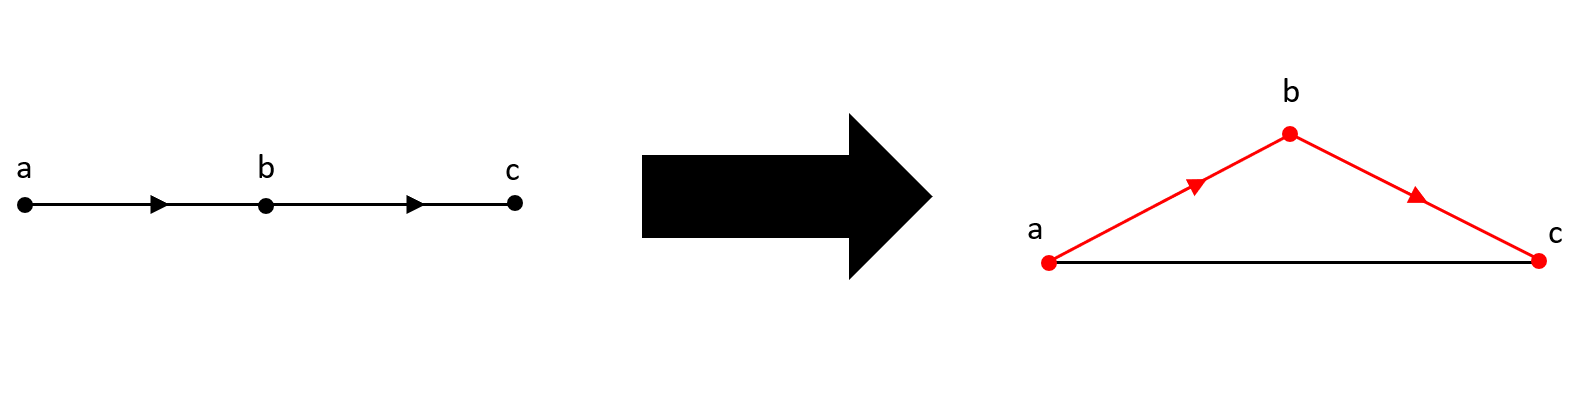
\includegraphics[width=\linewidth]{Dion's_Images2/complexint.png}}

i.e. we have $f:\mathbb{C} \rightarrow \mathbb{C}$?

Consider a parametrised integral with $a = -1, c = 1, f(z) = z^2$,
\begin{align*}
\frac{2}{3} =^? \int_{-1}^1 z^2 \mathrm{d}z &= \left\{ \int_{-1}^i + \int_i^1 \right \} z^2 \mathrm{d}z \\
&= \int_{-1}^i z^2 \mathrm{d}z + \int_{i}^1 z^2 \mathrm{d}z
\end{align*}
Let $z = \gamma_1(t) = -1 + t(1+i)$, $\gamma_1'(t) = 1 + i$ and $z = \gamma_2(t) = i + t(1-i)$, $\gamma_2'(t) = 1-i,$ for $0 \leq t \leq 1$. Then we have
\begin{align*}
\int_{-1}^1 z^2 \mathrm{d}z &=\int_{0}^1 [-1 + t(1+i)]^2(1+i) \mathrm{d}t + \int_{0}^1 [i + t(1-i)]^2(1-i) \mathrm{d}t \\
&=\ldots=\frac{2}{3}.
\end{align*}
While this is far from a complete proof, it does seem like equivalent integrals also exist in the same way for $f:\mathbb{C} \rightarrow \mathbb{C}$.
Note also that
\begin{align*}
\int_{-1}^1 z^2 \mathrm{d}z &= \frac{z^3}{3} \bigg\lvert_{z=1} - \frac{z^3}{3} \bigg\lvert_{z=-1} = \frac{2}{3} \\
&= F(1) - F(-1) \mbox{ using } F(z) = \frac{z^3}{3} \mbox{ so that } F'(z) = z^2 \mbox{ and}
\end{align*}
\begin{align*}
\int_{-1}^i z^2 \mathrm{d}z + \int_{i}^1 z^2 \mathrm{d}z &= F(i) - F(-1) + F(1) - F(i) \\
= F(1) - F(-1).
\end{align*}
Therefore, FTC seems to work for $f:\mathbb{C} \rightarrow \mathbb{C}$ too.

\subsection{Green's Theorem $\rightarrow$ Cauchy's Theorem}
Recall Green's Theorem from the Foundations of Applied Mathematics (FoAM) module:
\begin{thm}[Green's Theorem]
If $D$ is a region with finitely many (pairwise disjoint) regions removed from it,
$\partial D$ is the positively-oriented boundary of $D$ and $P, Q: \mbos{clos}(D) \rightarrow \mathbb{C}$ continuous with continuous partial derivatives, then 
$$\int_{\partial D}P \mathrm{d}x + Q \mathrm{d}y = \int\int_D \frac{\partial Q}{\partial x} - \frac{\partial P}{\partial y} \mathrm{d}x\mathrm{d}y.$$
\end{thm}
Region $D$ looks like this:

\centerline{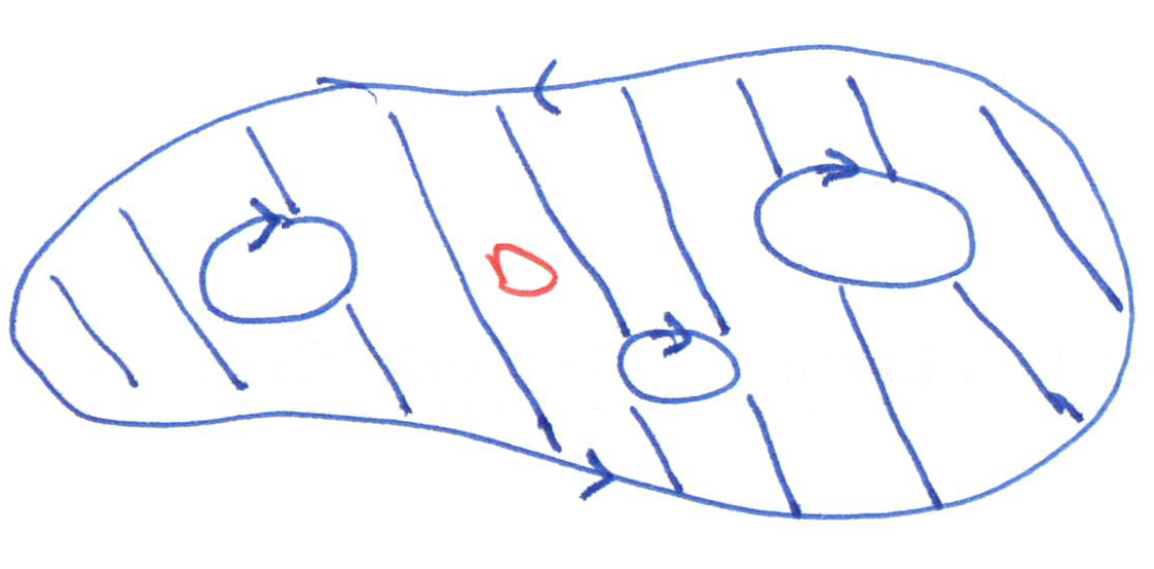
\includegraphics[width=\linewidth]{Dion's_Images2/greens.png}}

\begin{lem}[The Cauchy-Riemann Equations]
If $f$ is a complex-valued function and $f(x+iy) = u(x,y) + iv(x,y)$ for $u,v$ are real-valued functions and $x,y \in \mathbb{R}$,
then $u_x = v_y$ and $u_y = - v_x$ if and only if $f$ is analytic.
\end{lem}
For a proof of this lemma, take see the Complex Analysis module or check directly for any $f$ you care about.

\begin{thm}[Cauchy's Theorem]
If $\gamma = \partial D$ for $D$ is a region with finitely many regions removed and $f$ is analytic on an open set containing clos($D$), then
$$\int_\gamma f(z) \mathrm{d}z = 0.$$
\end{thm}
The idea for the proof of Cauchy's Theorem is that
\begin{align*}
\int_\gamma f(z) \mathrm{d}z &= \int_a^b [u(x(t), y(t)) + iv(x(t),y(t))](x'(t) + iy'(t))\mathrm{d}t \\
&= \ldots = \int_\gamma (u \mathrm{d}x - v \mathrm{d}y) + i\int_\gamma (v \mathrm{d}x + u \mathrm{d}y) \\
&= \int\int_D \frac{\partial}{\partial x}(-v) - \frac{\partial}{\partial y}(u) \mathrm{d}x\mathrm{d}y + i \int\int_D \frac{\partial}{\partial x}(u) - \frac{\partial}{\partial y}(v) \mathrm{d}x\mathrm{d}y \\
&\hspace{1pc}\mbox{(by applying Green's Theorem to each integral)} \\
&= 0 \mbox{ (by the Cauchy-Riemann equations)}.
\end{align*}
It seems like we dropped the criterion that $f$ has continuous derivatives, however, if $f$ is analytic on a region containing $\lambda$, then $f^{(n)}(\lambda)$ exists and is continuous for all $n\in\mathbb{N}$.

\medskip\textbf{Example 1:} Consider the following diagram:

\centerline{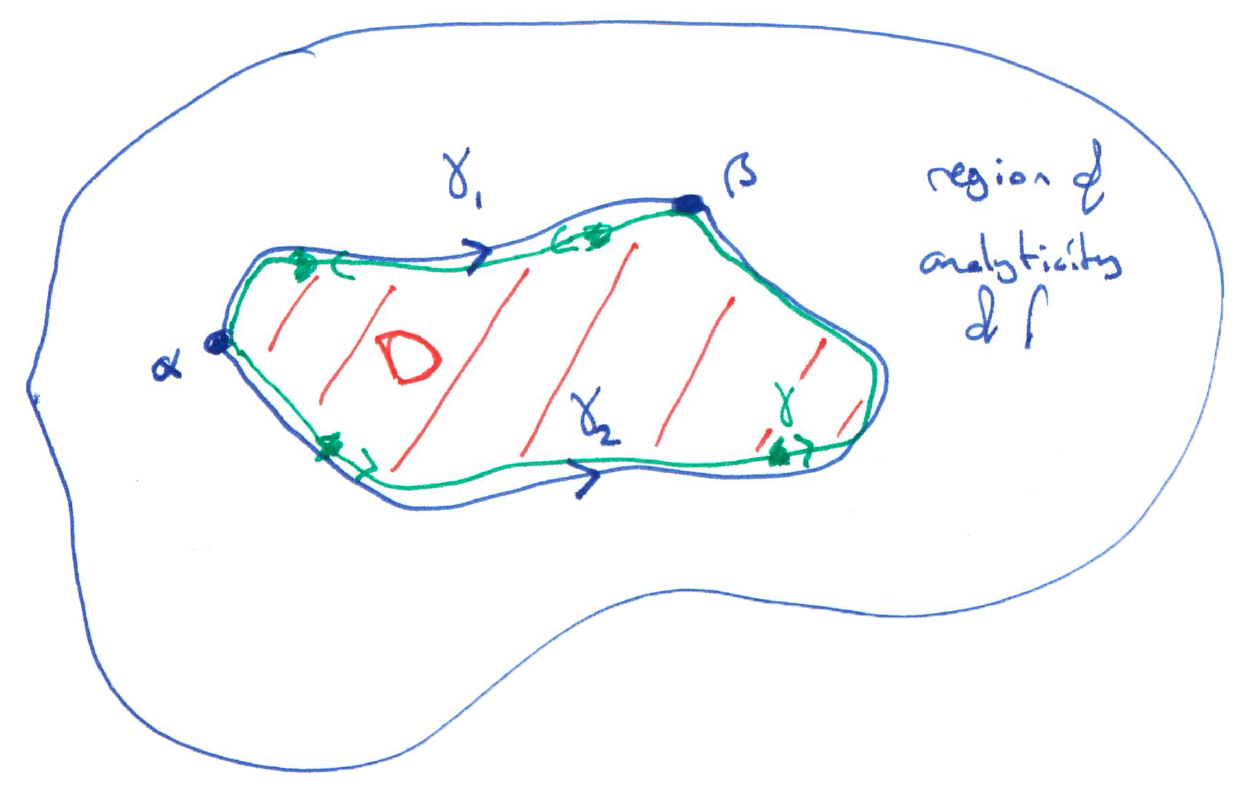
\includegraphics[width=\linewidth]{Dion's_Images2/eg1.png}}

let $\gamma = \partial D = [-\gamma_1] \cup [\gamma_2]$.
By Cauchy's Theorem,
$$\int_\gamma f(z) \mathrm{d}z = 0.$$
Since $\gamma$ is the same path as $\gamma_1$ in the opposite direction followed by $\gamma_2$, equivalence of integrals follows with
$$\left\{-\int_{\gamma_1} + \int_{\gamma_2}\right\}f(z) \mathrm{d}z = 0,$$
which implies that
$$\int_{\gamma_1}f(z) \mathrm{d}z = \int_{\gamma_2}f(z) \mathrm{d}z,$$
i.e. these integrals are equivalent despite lying on different paths!

So if $F' = f$ and $F$ is continuous, using the Fundamental Theorem of Calculus, the integral of $f$ over $\gamma_1$ is path-independent:
$$\int_{\gamma_1}f(z) \mathrm{d}z = F(\beta) - F(\alpha);$$
we only need to care about the endpoints of the integration, just like for the integration of real-valued functions!

\medskip\textbf{Example 2:} Consider the following diagram:

\centerline{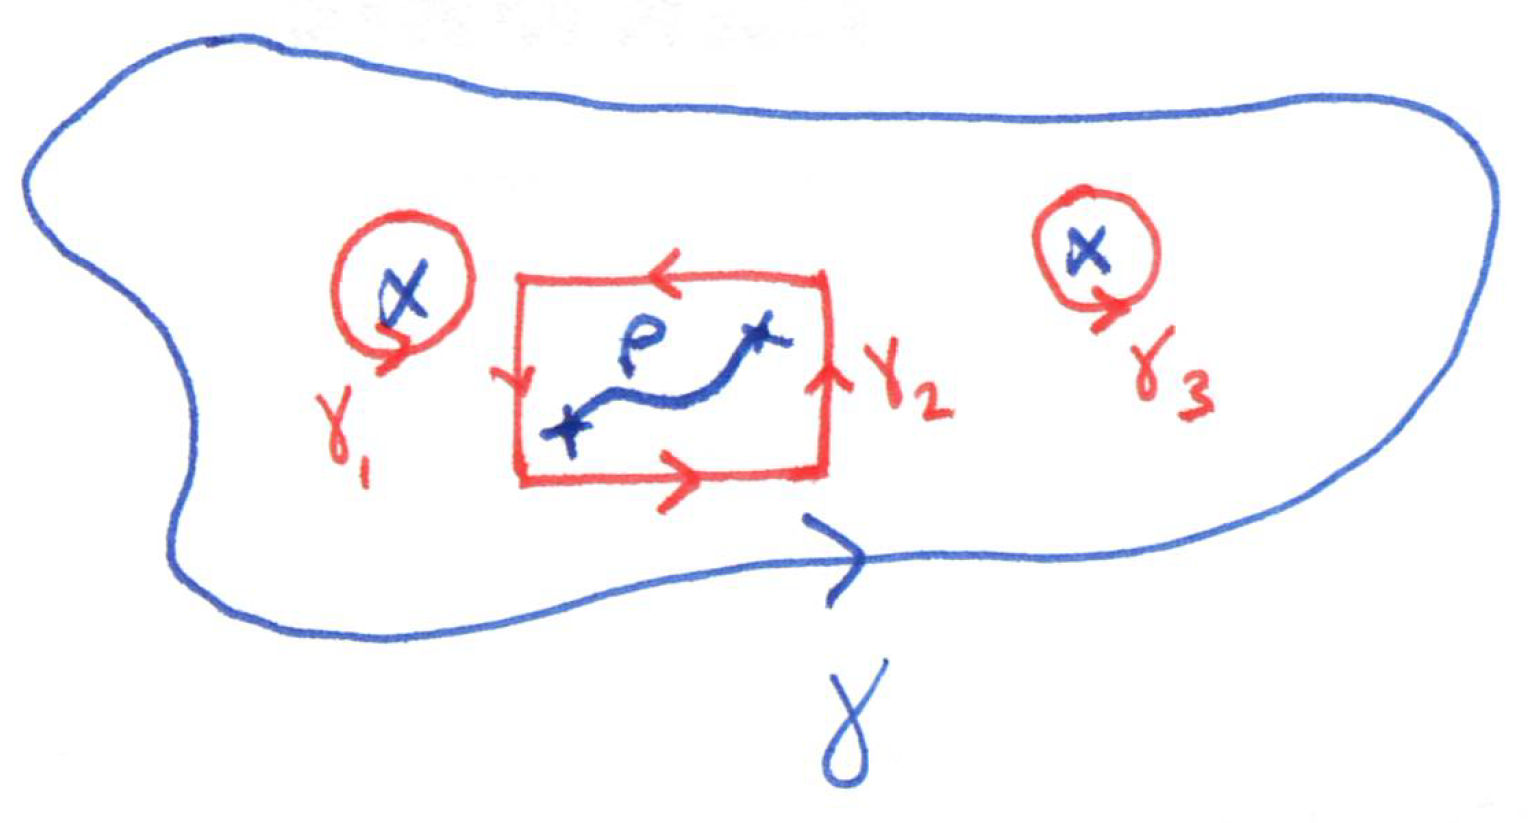
\includegraphics[width=\linewidth]{Dion's_Images2/eg2.png}}

Let $f$ be analytic everywhere except at $x$ and on $p$, then
$$\int_\gamma f(z) \mathrm{d}z = \int_{\gamma_1} f(z) \mathrm{d}z + \int_{\gamma_2} f(z) \mathrm{d}z + \int_{\gamma_3} f(z) \mathrm{d}z.$$
These integrals are easier to evaluate (at least numerically) because they can be parametrised using simple circular/polygonal paths.

\subsection{Complex Integrals to $\infty$ (Improper Complex integrals)}

\begin{lem}[Sub-lemma for Jordan's lemma]
$$\forall R > 0, \forall x > 0, \int_0^\pi e^{-Rx\sin(\theta)} \mathrm{d}\theta \leq \frac{\pi}{Rx}$$
\end{lem}

\begin{proof}
The graph

\centerline{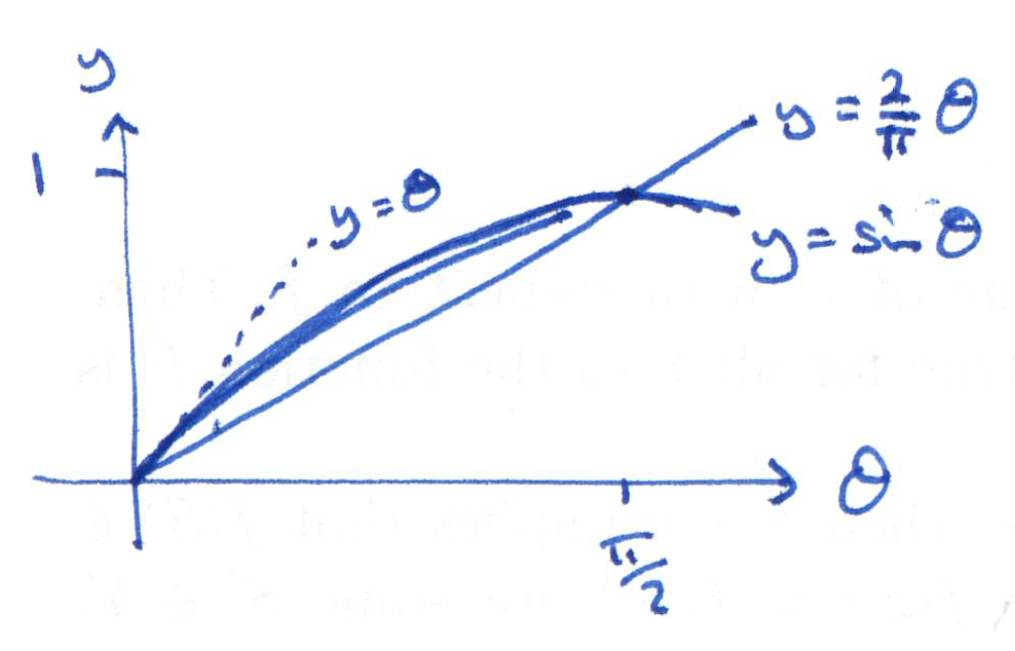
\includegraphics[width = \linewidth]{Dion's_Images2/sublemma.png}}

shows that 
\begin{align*}
\forall \theta \in \left[0, \frac{\pi}{2}\right], &\sin(\theta) \geq \frac{2}{\pi}\theta \geq 0 \\
&\implies -Rx\sin(\theta) \leq \frac{-2}{\pi}Rx\theta \leq 0 \\
&\implies 0 \leq e^{-Rx\sin(\theta)} \leq e^{-\frac{2}{\pi}Rx\sin(\theta)} \leq 1.
\end{align*}
$$\int_0^\pi e^{-Rx\sin(\theta)} \mathrm{d}\theta = \int_0^{\frac{\pi}{2}} e^{-Rx\sin(\theta)} \mathrm{d}\theta + \int_{\frac{\pi}{2}}^\pi e^{-Rx\sin(\theta)} \mathrm{d}\theta.$$
Perform a change of variables in the second integral with $t = \pi - \theta$, then
$$\int_0^{\frac{\pi}{2}} e^{-Rx\sin(\theta)} \mathrm{d}\theta + \int_{\frac{\pi}{2}}^0 e^{-Rx\sin(\pi - t)}(-1) \mathrm{d}t = \ldots = 2\int_0^{\frac{\pi}{2}} e^{-Rx\sin(\theta)} \mathrm{d}\theta,$$
this still cannot be integrated analytically, however, we can now use the inequality. Note that the integral is everywhere positive. Therefore,
$$\int_0^\pi e^{-Rx\sin(\theta)} \mathrm{d}\theta \leq 2\int_0^{\frac{\pi}{2}} e^{-\frac{2}{\pi}Rx\theta} \mathrm{d}\theta = 2(1-e^{-Rx})\frac{\pi}{2Rx} \leq \frac{\pi}{Rx}$$
which completes the proof.
\end{proof}

\begin{lem}[Jordan's lemma]
Suppose $R_0 \geq 0$ and $0 \leq \theta_1 < \theta_2 \leq \pi$.
Let $\sigma_R$ = circular arc$\{Re^{i\theta}: \theta \in [\theta_1, \theta_2]\}.$
Suppose $f$ is a continuous, complex-valued function on $\{Re^{i\theta}: \theta \in [\theta_1, \theta_2], R \geq R_0\}.$
Let $M(R) = \max\{\abs{f(z)}: z \in \sigma_R\}.$
Suppose $\lim_{R\rightarrow\infty} M(R) = 0$.
Then, $$\forall x > 0, \lim_{R\rightarrow\infty} \int_{\sigma_R} e^{ixz} f(z) \mathrm{d}z = 0.$$
\end{lem}
The following is a diagram showing Jordan's lemma:

\centerline{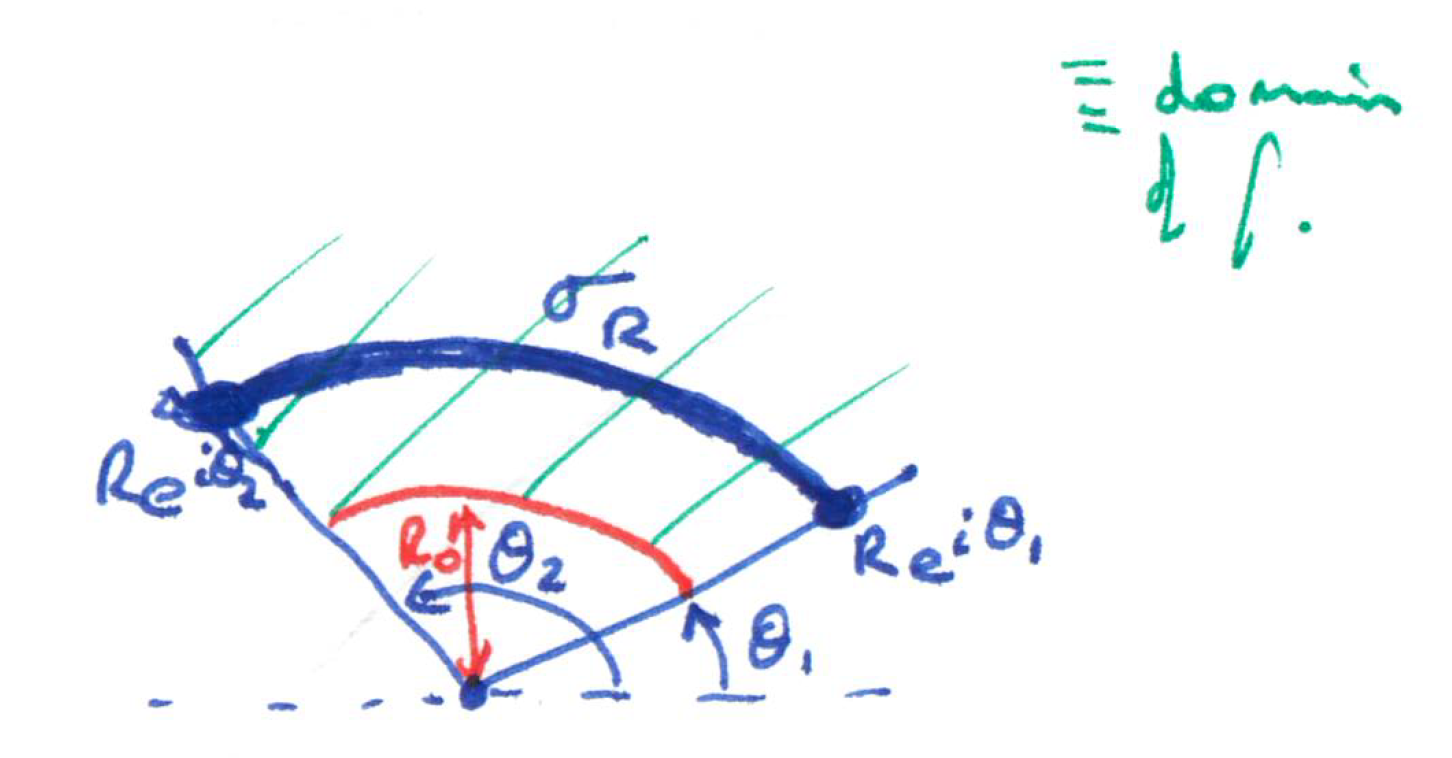
\includegraphics[width=\linewidth]{Dion's_Images2/jordanlem.png}}

Informally, Jordan's lemma states that ``Even though the arc $\sigma_R$ gets infinitely long, the decay of the maximum of $\abs{f(z)}$ on the arc,
together with the oscillatory nature of $e^{ixz}$, is enough to make the integral tend to 0". 
This is the same kind of result as the Riemann-Lebesgue lemma.

\begin{proof}
We want to show that an integral has a limit of zero, so it is equivalent to show its modulus has a limit of zero.
Parametrise $\sigma_R$ by $\gama(\theta) = Re^{i\theta} for \theta \in [\theta_1, \theta_2]$. Then, by the sub-lemma,
\begin{align*}
\abs{\int_{\sigma_R} e^{ixz} f(z) \mathrm{d}z} &= \abs{\int_{\theta_1}^{\theta_2} e^{ixRe^{i\theta}}f(Re^{i\theta}) Rie^{i\theta} \mathrm{d}\theta} \\
&\leq R\int_{\theta_1}^{\theta_2} \abs{e^{ixRe^{i\theta}}}\abs{f(Re^{i\theta})} \abs{ie^{i\theta}} \mathrm{d}\theta \\
&\leq R\int_{\theta_1}^{\theta_2} e^{-xR\sin(\theta)} M(R) \mathrm{d}\theta \\
&= RM(R)\int_0^\pi e^{-xR\sin(\theta)} \mathrm{d}\theta \\
&\leq RM(R)\frac{\pi}{xR} = \frac{\pi M(R)}{x} \rightarrow 0 \mbox{ as } R \rightarrow \infty.
\end{align*}
\end{proof}

\medskip\textbf{Example 3:}
$f(x) = \frac{x}{x^2 + 1}$. Evaluate 
$$I = \int_{-\infty}^{\infty} f(x) \cos(x) \mathrm{d}x.$$
Note that 
$$I = \mbox{Re}\left(\int_{-\infty}^{\infty} f(x)e^{ix} \mathrm{d}x \right) = \mbox{Re}\left(\lim_{R \rightarrow \infty}\int_{-R}^{R} f(x)e^{ix} \mathrm{d}x \right).$$
Extend function $f$ to $\mathbb{C}$ (or at least to clos($\mathbb{C}^+$)) except $f$ is not defined at $x = i$ (and $x = -i$, though that does not matter).
Let $R \geq 2 = R_0$ (so we enclose $i$) and $\gamma_R = \sigma_R \cup [-R,R]$:

\centerline{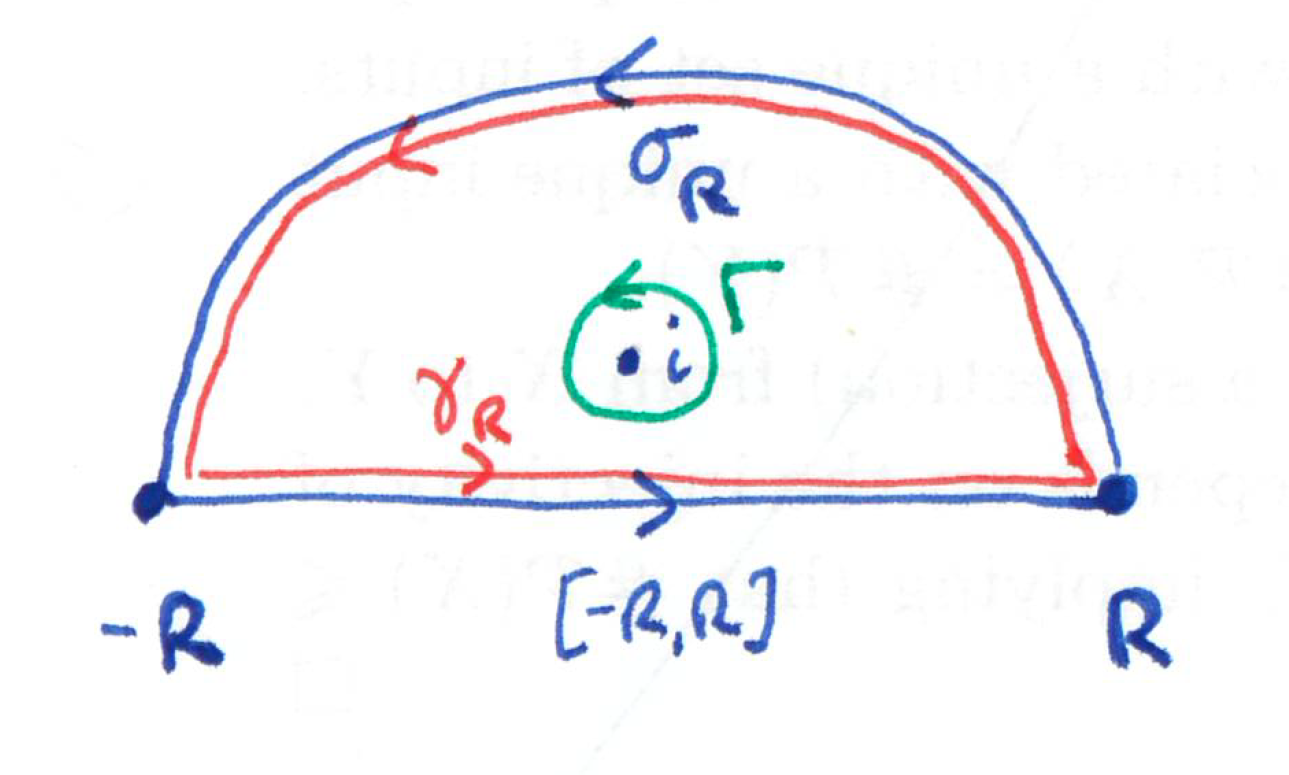
\includegraphics[width=\linewidth]{Dion's_Images2/eg3.png}}

Note that $f$ is analytic in all $\mathbb{C}$ except at $\pm i$.
Therefore,
\begin{align*}
\forall R \geq 2, \int_\Gamma f(z) e^{iz} \mathrm{d}z &= \int_{\gamma_{R_0=2}}f(z) e^{iz} \mathrm{d}z \mbox{ by Cauchy's theorem} \\
&= \int_{\gamma_R} f(z) e^{iz} \mathrm{d}z \mbox{ by another application of Cauchy's theorem} \\
&= \int_{-R}^R f(z) e^{iz} \mathrm{d}z + \int_{\sigma_R} f(z) e^{iz} \mathrm{d}z.
\end{align*}

But
$$\abs{f(Re^{i\theta})} = \frac{R\abs{e^i\theta}}{\abs{R^2 e^2i\theta + 1}} \leq \frac{R}{R^2 - 1} \rightarrow 0 \mbox{ as } R \rightarrow \infty.$$
Therefore, $\forall R \geq 2,$
\begin{align*}
&\int_{\sigma_R} f(z) e^{iz} \mathrm{d}z = 0 \mbox{ by Jordan's lemma} \\
&\implies \int_{-R}^R f(z) e^{iz} \mathrm{d}z = \int_\Gamma f(z) e^{iz} \mathrm{d}z \\
&\implies \int_{-\infty}^\infty f(x) \cos(x) \mathrm{d}x = \mbox{Re}\left(\int_\Gamma f(z) e^{iz} \mathrm{d}z\right).
\end{align*}
In this way we replaced an improper integral with an integral about a circular contour.
This would be easy to calculate numerically.
Even better, using Cauchy's residue calculus (see Complex Analysis or FoAM modules),
this integral can be calculated very easily.

\medskip\textbf{Example 4:}
Let $f$ be analytic on $\mathbb{C}$ except at each $X$ where it is undefined.
$\abs{f(z)} \rightarrow 0$, uniformly in arg$(z)$, as $z \rightarrow \infty$ with $\{Re^{i\theta}: R > R_0, \theta \in [\frac{\pi}{4}, \frac{3\pi}{4}]\}$.
Consider the diagram:

\centerline{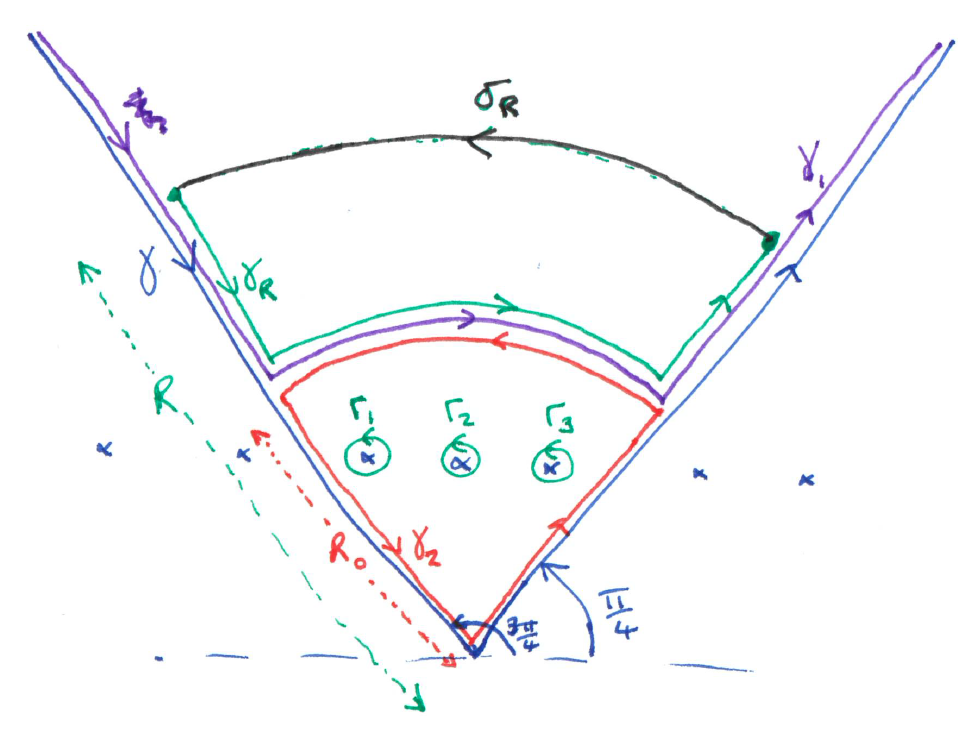
\includegraphics[width=\linewidth]{Dion's_Images2/eg4.png}}

we have,
\begin{align*}
\int_\gamma f(z) e^{izx} \mathrm{d}z &= \int_{\gamma_1} f(z) e^{izx} \mathrm{d}z + \int_{\gamma_2} f(z) e^{izx} \mathrm{d}z \\
&= \lim_{R\rightarrow \infty} \int_{\gamma_R} f(z) e^{izx} \mathrm{d}z + \left\{ \int_{\Gamma_1} + \int_{\Gamma_2} + \int_{\Gamma_3}\right\} f(z) e^{ixz} \mathrm{d}z \mbox{ by Cauchy's theorem}.
\end{align*}
However,
\begin{align*}
\lim_{R\rightarrow \infty} \int_{\gamma_R} f(z) e^{izx} \mathrm{d}z &= \lim_{R\rightarrow \infty}\left[\left\{\int_{\gamma_R} + \int_{\sigma_R}\right\} f(z) e^{ixz} \mathrm{d}z - \int_{\sigma_R} f(z) e^{ixz} \mathrm{d}z \right] \\
&= \lim_{R\rightarrow \infty}\left[ 0 - \int_{\sigma_R} f(z) e^{ixz} \mathrm{d}z \right] \mbox{ by Cauchy's theorem} \\
&= 0 \mbox{ by Jordan's lemma}.
\end{align*}
Therefore,
$$\int_\gamma f(z) e^{izx} \mathrm{d}z = \left\{ \int_{\Gamma_1} + \int_{\Gamma_2} + \int_{\Gamma_3}\right\} f(z) e^{ixz} \mathrm{d}z.$$
Once again we have transformed an improper complex integral into a sum of finite circular contour integrals which are much easier to evaluate especially with the use of residue calculus.